\documentclass[11pt]{article}
\pagestyle{headings}

\usepackage{fullpage}
\usepackage{graphicx}
\usepackage{sidecap}
\usepackage{subfig}
\usepackage{float}


\title{Tweet District Design Document}
\author{Victor Frolov}
\graphicspath{ {images/} }


\begin{document}
\maketitle

\section{Introduction}
Tweet District is an app that lets you find and interact with hundreds of tweets in your area (or any location of your choosing), and provides a way to find out about parties, local events, sales, promotions, and job hirings, and its all shown on a map. Although it is currently a web app, its use would be far greater on a mobile device. The purpose of this paper is to come up with a dream interface for this app, and use it as a guide during future development. Interaction design principles and theories are imperative to its development, and will range from usability measures, mental models, and many others.


\section{Landing Page}
Once a user downloads and opens the app, they will be greeted with a landing page with the logo, and app name that takes up a third of the screen. There will be one large button that allows the user to login to their existing Twitter account (which will allow them to interact with the tweets, such as retweeting, sending direct messages, etc). Below the button will simply be tappable text that says "Use as Guest", allowing users to use the app without a Twitter account. The logo, app name, button and text will be over a background color that will stay true to the app's theme. The background color will have opacity, and behind it there will be animations of users tweeting, partying, and shopping. These animations would be slightly fuzzy. Please see figure~\ref{fig:loginMock}.

\begin{figure}[H]
    \centering
    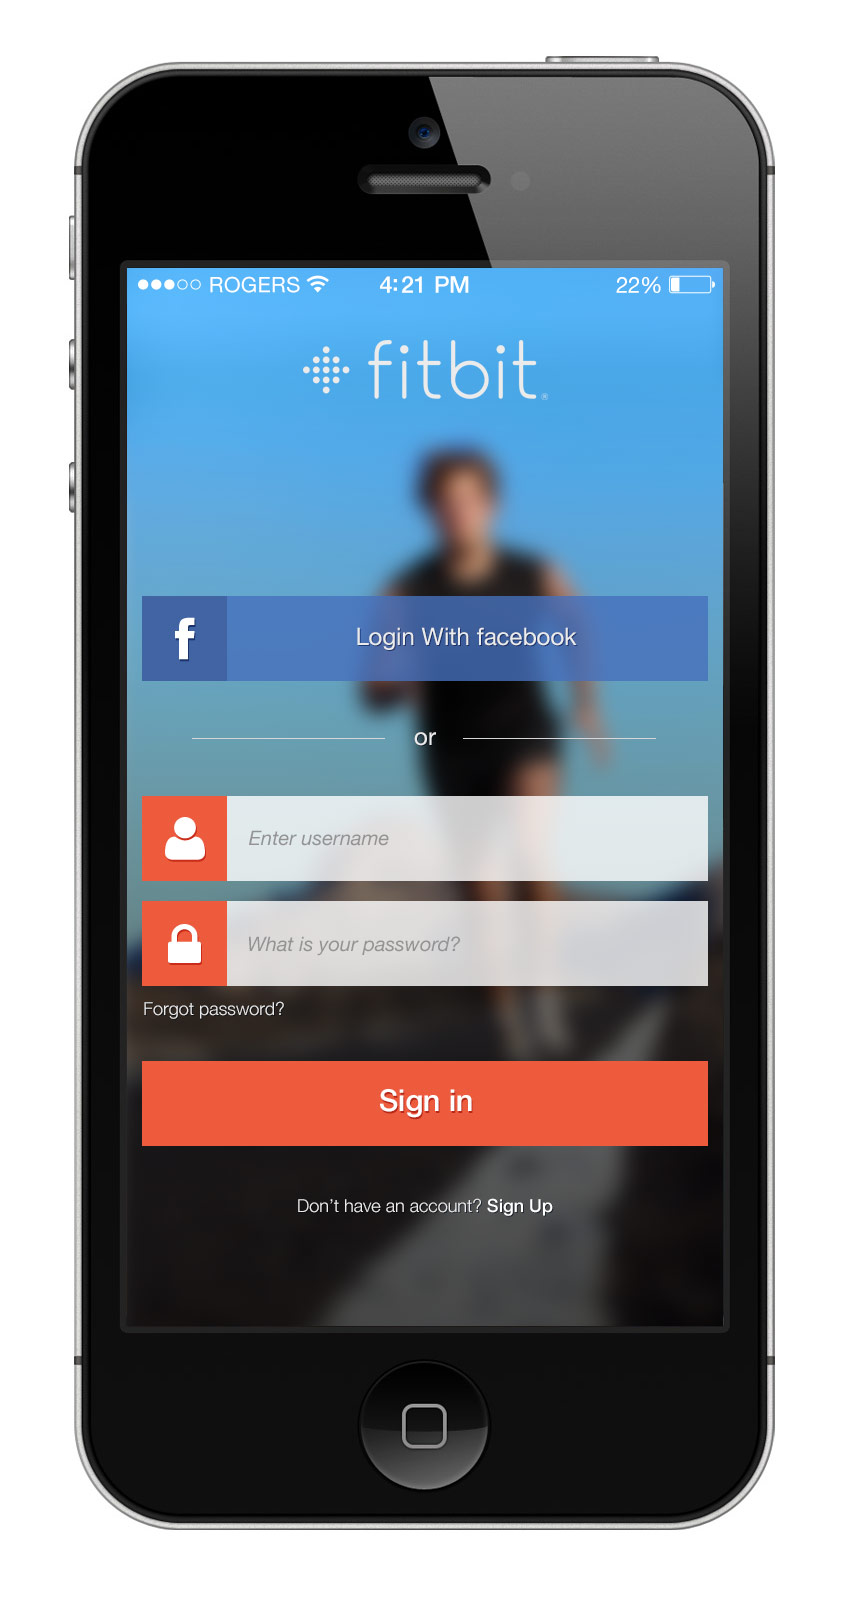
\includegraphics[width=7cm]{loginIdea}
    \caption{Landing/Login Page Example}  
    \label{fig:loginMock}          
\end{figure}

The "Login with Facebook" would be moved down to the "Sign in" location, and all other boxes and buttons would be removed. Login with Facebook would be changed to Twitter, and below it there would be the aforementioned text of "Use as Guest". The Fitbit logo and Fitbit name would be of course replaced with the Tweet District Logo and Tweet District name. The man running in the background would be replaced with a sequence of short videos.

\section{Main Functionality}
The app's main functionality can be broken up into three sections:
\begin{itemize}
\item Searching
\item Displaying the tweets on a map
\item Displaying the tweets in an ordered fashion that is useful
\end{itemize}

Once a user either logs in to their Twitter account, or continues as guest, they would be greeted with the search page. All pages, excluding the landing/home page, would have a navigational dock with buttons on the bottom of the screen, like in iOS's native Podcast app. Please see Figure~\ref{fig:navButtons} below.

\begin{figure}[H]
    \centering
    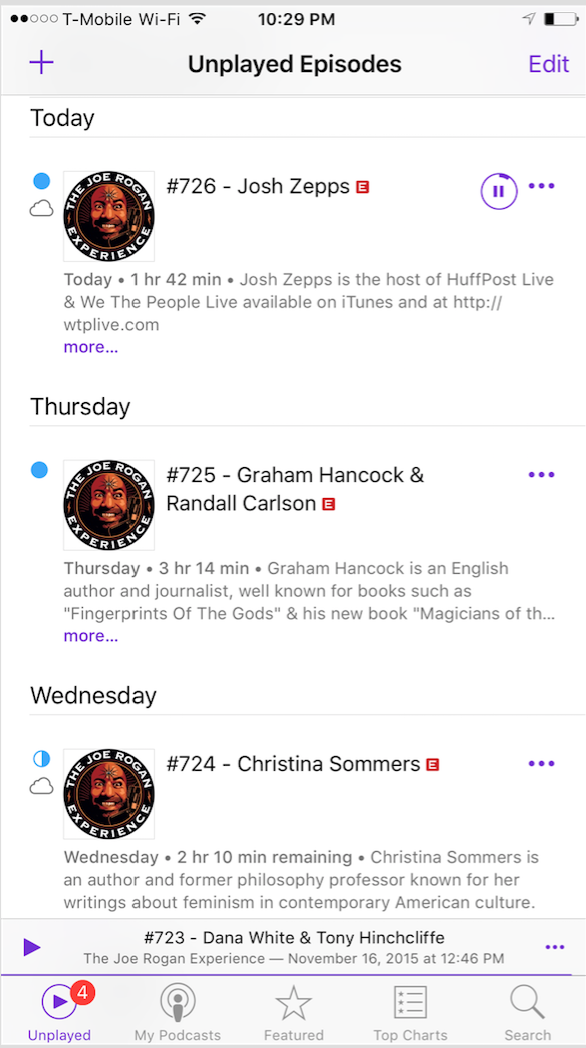
\includegraphics[width=7cm]{navButton}
    \caption{Navigational Buttons at the bottom of the Page}
    \label{fig:navButtons}                
\end{figure}

The buttons would be Search, Tweets, Map, Profile and a Sandwich. Search, Tweet, Map and Profile would bring the user to the respective page, allowing them to search, see found tweets, see tweets on a map, and access their saved tweets where they can interact with them (such as retweeting, direct messaging, sharing, etc). The sandwich button would be similar to Figure~\ref{fig:searchTemplate} (b) but the sliding animation would occur from the right side, towards the left. Please see the Advanced Search section for more information on the sliding animation. Once the slide occurs, the user would have the ability to be directed to an FAQ page, the ability to log out, custom updates, and the ability to send a message to the response team.

The navbar button on the active page would glow, just as in Figure~\ref{fig:navButtons} where all the inactive buttons would not, visually showing the user where they are in the app.

\subsection{Searching}
Before diving into the search functionality, it is important to note that all of the suggestions and current limitations are directly correlated to the usability metric of efficiency. The process of searching should be quick, simple and almost instantaneous, with optional extra steps for extra precision and only if the user demands it. It should not be forced upon them.

\subsubsection{Simplified Search}
When I tried using the app on my mobile device when I was out and about with some friends, we found that there were a few issues impeding us from having a great experience. The first issue was having to type in a search word, check the current location box, and tapping search each and every single time we tried looking up something around us. See Figure~\ref{fig:SearchSimple} (a).

\begin{figure}[H]
    \centering
    \subfloat[Current Search Appearance]{{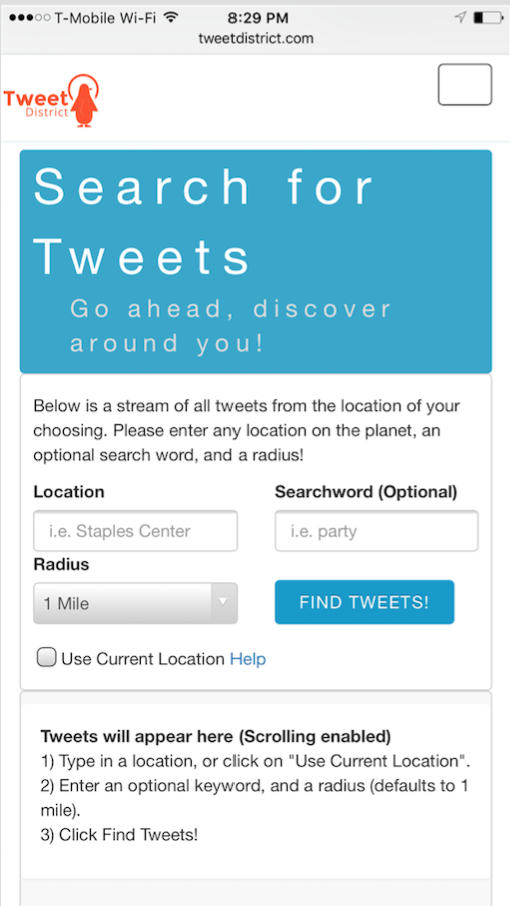
\includegraphics[width=7cm]{currentSearch} }}
    \qquad
    \subfloat[Simplified Search Appearance]{{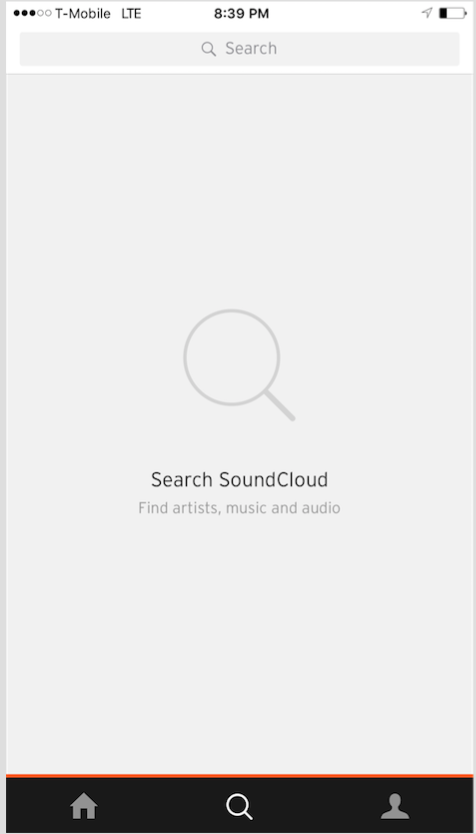
\includegraphics[width=7cm]{newSearch} }}
    \caption{Old Search and New Search Template}
    \label{fig:SearchSimple}          

\end{figure}

In order to overcome the first hurdle of having to repetitively do a series of steps (we tried looking up about 10 keywords to find events around us, and although it ultimately worked, the process was arduous), a simplified search, as in figure~\ref{fig:SearchSimple} (b), would be ideal. It would be preset to search a certain radius from the user's current location. That way they simply just type in a word or sequence of words, and hit search. There should be very little distraction and filler, so that they know exactly what to do just by glancing at the screen. The simpler, the better.

\subsubsection{Advanced Search}
Since the app is all about searching, it is important to have advanced search still available. Text near the top that says ``More Search Options", once pressed, would animate the app to swipe to the right, similar to Yahoo Fantasy Football's top left sandwich button. See Figure~\ref{fig:searchTemplate}.

\begin{figure}[H]
    \centering
    \subfloat[Before button was pressed]{{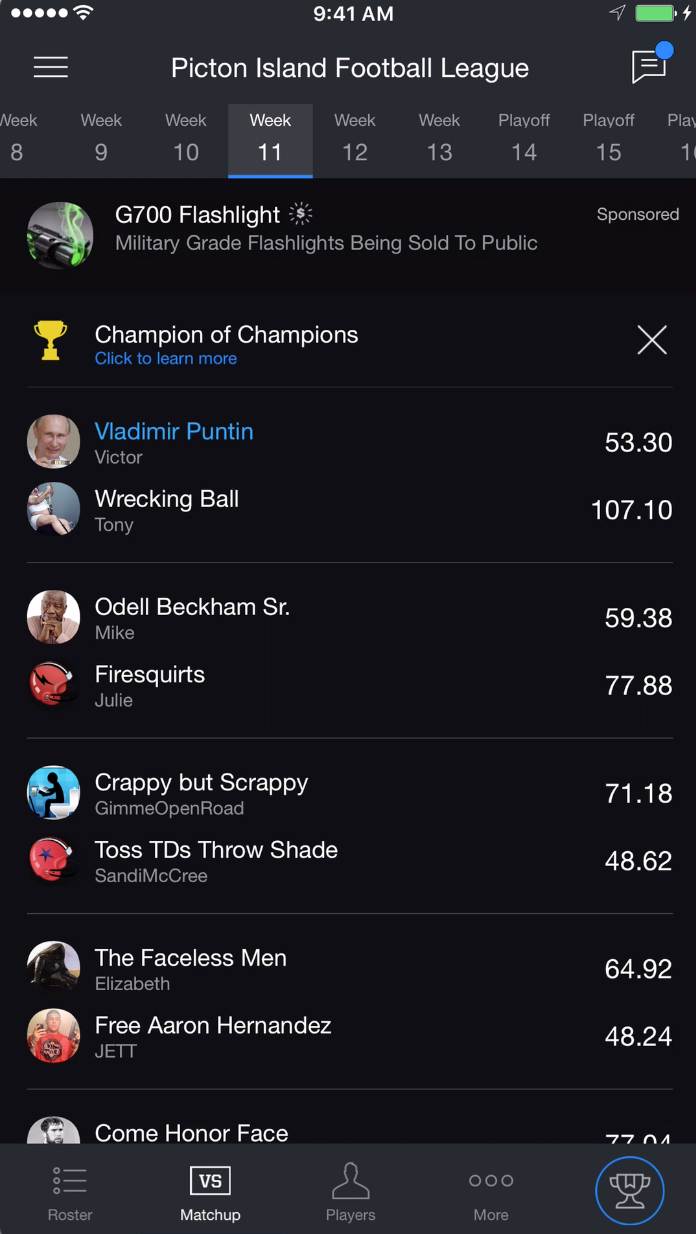
\includegraphics[width=7cm]{beforeSearch} }}
    \qquad
    \subfloat[After button was pressed]{{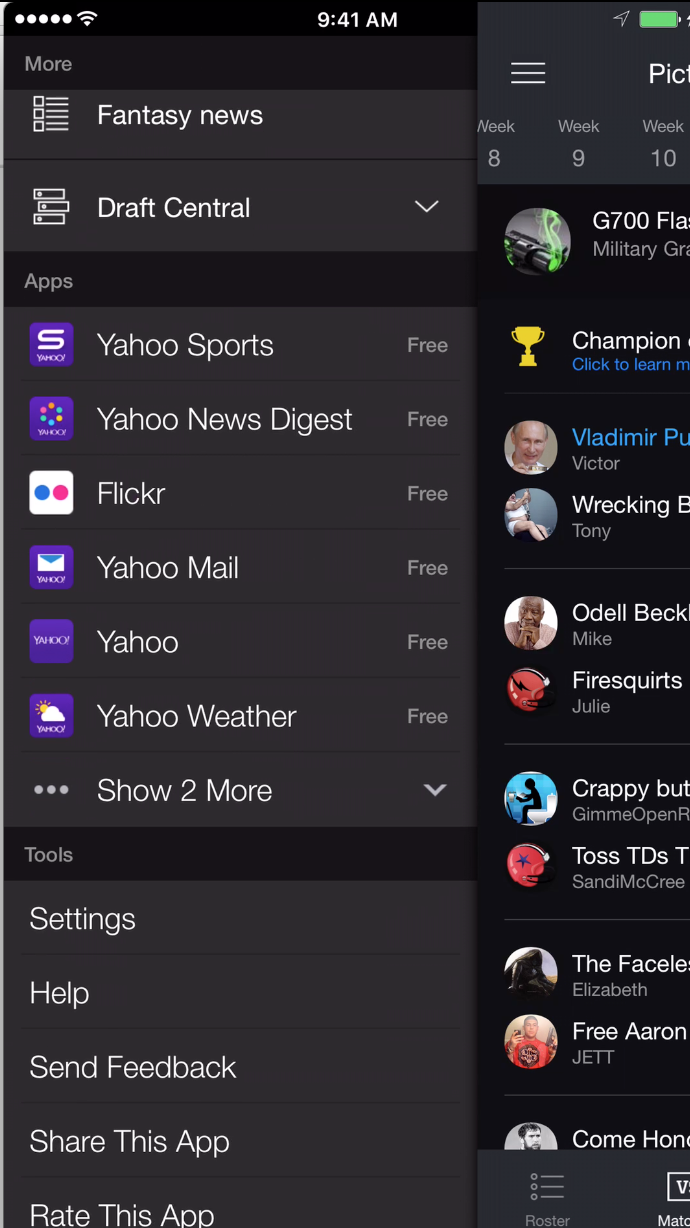
\includegraphics[width=7cm]{afterSearch} }}
    \caption{Advanced Searching}
    \label{fig:searchTemplate}
\end{figure}

So before the button was pressed, the search tab would simply look like Figure~\ref{fig:SearchSimple} (b), and after the button is pressed, it would slide everything on the screen to the right, and would look close to what Figure~\ref{fig:searchTemplate} (b) looks like. But of course, instead of displaying Yahoo information, it would show optional fields such as: 

\begin{itemize}
\item Custom radius
\item Custom location (using geocoding and geodecoding)
\item Excluding certain users (this was a small issue where sometimes a user would tweet 20 times about the same event) 
\item Enabling predefined searches
\item Searching within a date range (so that a tweet from a few weeks ago that is no longer relevant doesn't show up)
\item Only displaying one tweet per user
\item Excluding words and hashtags. 
\end{itemize}

The ability to save what the user input and make it become the ``default" search should also be implemented. That way if the user always looks for ``party" within a 3 mile radius of a specific location, they can do that with a single tap. Tapping on show less would slide the search back onto the screen, and would again look like figure~\ref{fig:SearchSimple} (b) above. The purpose of the animation is to draw attention to what is changing. 

\subsubsection{Predefined Searches}

One final feature, which again would be to streamline searching, would be predefined searches. The user enables ``predefined searches", in the advanced search options. This would then turn the search bar into a dropdown list of predefined searches. So, for example, if they were to select ``party" in the dropdown list and hit search, it would automatically search the API for multiple keywords predefined by the app. Twitter's API allows the use of ``OR" to string together multiple searches, so a potential combination could be ``party OR frat OR houseparty OR happyhour OR bar OR club". Of course, custom predefined searches should also be implemented so that a user can look up series of words without having to type them fully out each time they do a search. Approximately 5 categories would be built in (party, events, sales, hiring, nightlife), and a dozen custom searches can be saved to the list. The user must be logged in to their Twitter account in order to save custom searches, and would be prompted to do so if they are not logged in.



\subsubsection{Twitter's API Get/Searches Limitations}

As excellent as Twitter's API is, it has some limitations from Tweet District's perspective. They have the ability to ignore a user ID's tweets from showing up in the array results, but, the ID must be known beforehand. Unfortunately, Twitter does not have the ability to cap or ignore users that have posted more than ``x" tweets on a specific topic. This is a problem because, Twitter allows up to 100 tweets to be returned, and if there is a user spamming a certain topic, there is no clean way to ignore their tweets. One way would be to simply keep track of unique user ID's, and once there is repetition, to not append that tweet to the body, but of course, this would cause less than 100 tweets to be displayed. So if a user posted 60 times, and there was a total of 100 tweet results, only 41 tweets would be displayed. A workaround would be to make an initial call, track the amount of unique ID's, and if a user, for example, has tweeted more than 5 or 10 times on a topic, to then do a second search, and ignore specifically his username in that search, for a more unique return.


\subsection{Map}
The map section would show a map with markers dropped that represent the location of every tweet found by the API. The way the app currently appears on a mobile device is very difficult to navigate, as it takes almost the full screen width. Scrolling to and away from the map was difficult, since when the user tries to scroll down the page but does so by putting their finger within the map box boundary, he would zoom in or out of the map. There was about a quarter inch of space both to the left and right of the map that allowed the user to scroll the page.  See Figure~\ref{fig:mapProblem} below. Navigating between the map that had markers for all the tweets, and the box that displayed all the tweets in list form did not feel intuitive, and was tedious. This would of course be solved with separating Search, Tweets, and Map into their own pages with the nav bar on the bottom for easy navigation.

\begin{figure}[H]
    \centering
    \subfloat[Current Map layout]{{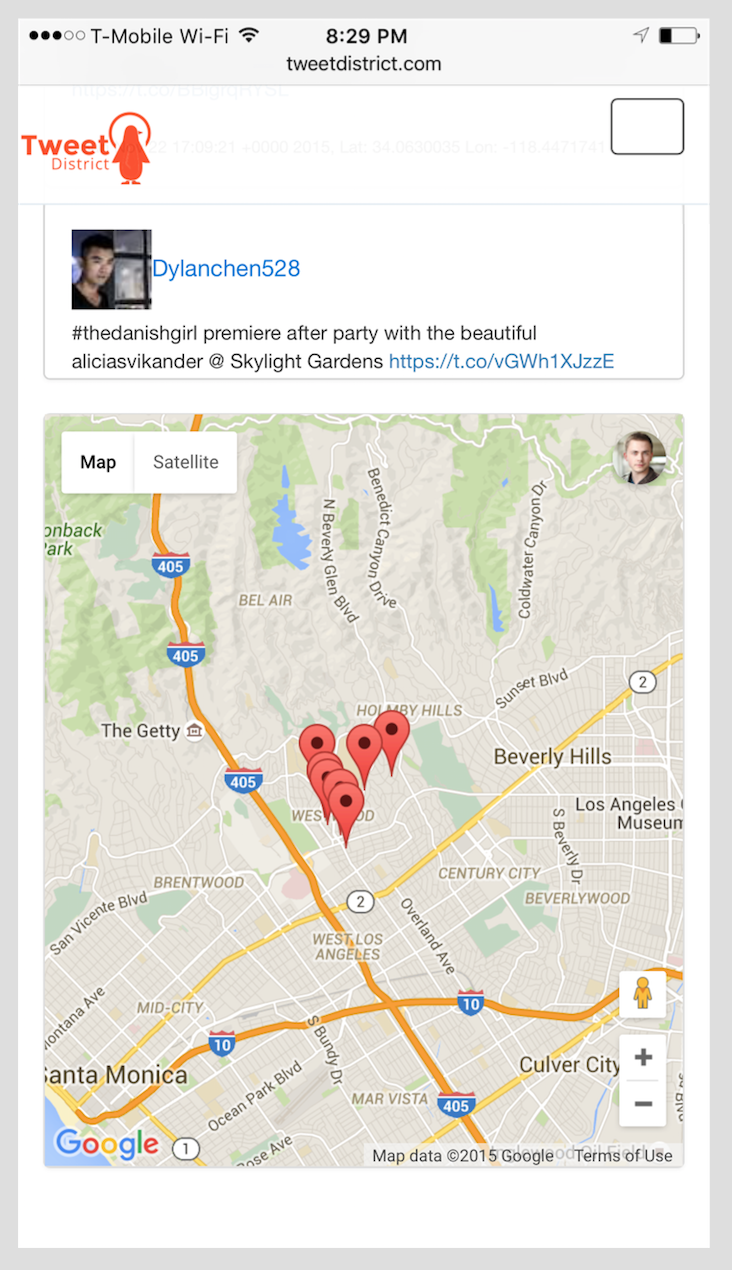
\includegraphics[width=7cm]{mapProblem} }}
    \qquad
    \subfloat[Another image of Map/Tweet layout]{{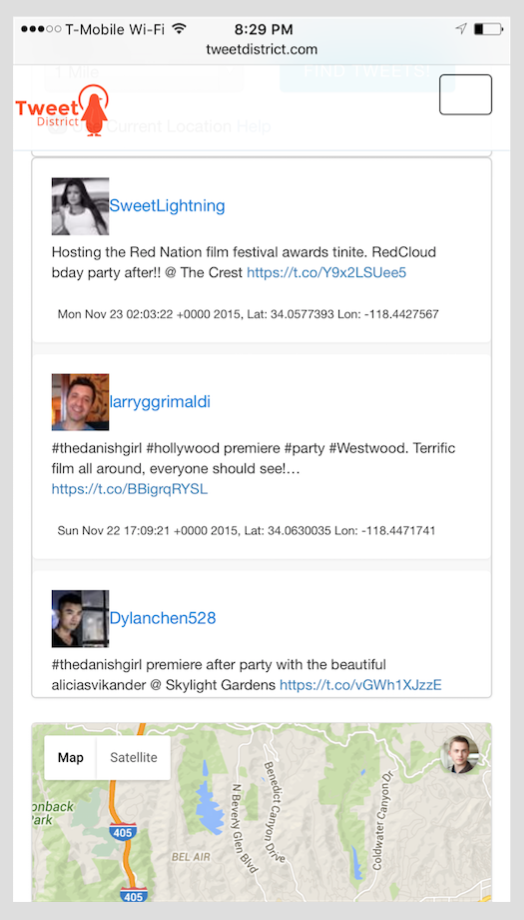
\includegraphics[width=7cm]{mapProblem2} }}
    \caption{Advanced Searching}
    \label{fig:mapProblem}
\end{figure}

The grey boxes engulfing the two above images are to show what is not on the screen. So, the user would have to put their finger far left or far right on the screen, in that narrow white gap, to navigate the page without zooming on the map, or scrolling through the displayed tweets. In the app version of Tweet District, when the user is on the map page, the map would take up the entire screen, aside for of course the navbar on the bottom of the device.

\subsubsection{Markers Storing Data}
Currently, the markers cannot be interacted with. Each marker should (and will) store the data of a tweet, so that when it is pressed on, it displays the user, and what they tweeted. It is hard to give an estimate of what the box width and length would be, but it should be large enough to display sufficient information, and small enough not to take up too much room on the mobile device. Some tweets would be cut off due to them being too long, or if they contain an image, and the cut off would be displayed with an ellipsis. Pressing anywhere on the box would make the box animate and get larger, displaying all of the information. When the box is larger and displaying all of it's information, the users would also be able to press on a user ID to go to their Twitter page, press on links to go wherever they link to, retweet the tweet, star it, create a new tweet with the same hashtag, and direct message the user who tweeted. Pressing again would make the box shrink to it's original size (as long as the user does not press on a link or a user ID). Each box will have one of their edges with a small triangular extension, to indicate which tweet the box is tied to.

Below is an example of how a marker would contain data. This would be the box in it's larger form. It is a screenshot of Padmapper, and a clicked marker that displays information about a room being leased. See figure~\ref{fig:markerDisplay}.

\begin{figure}[H]
    \centering
    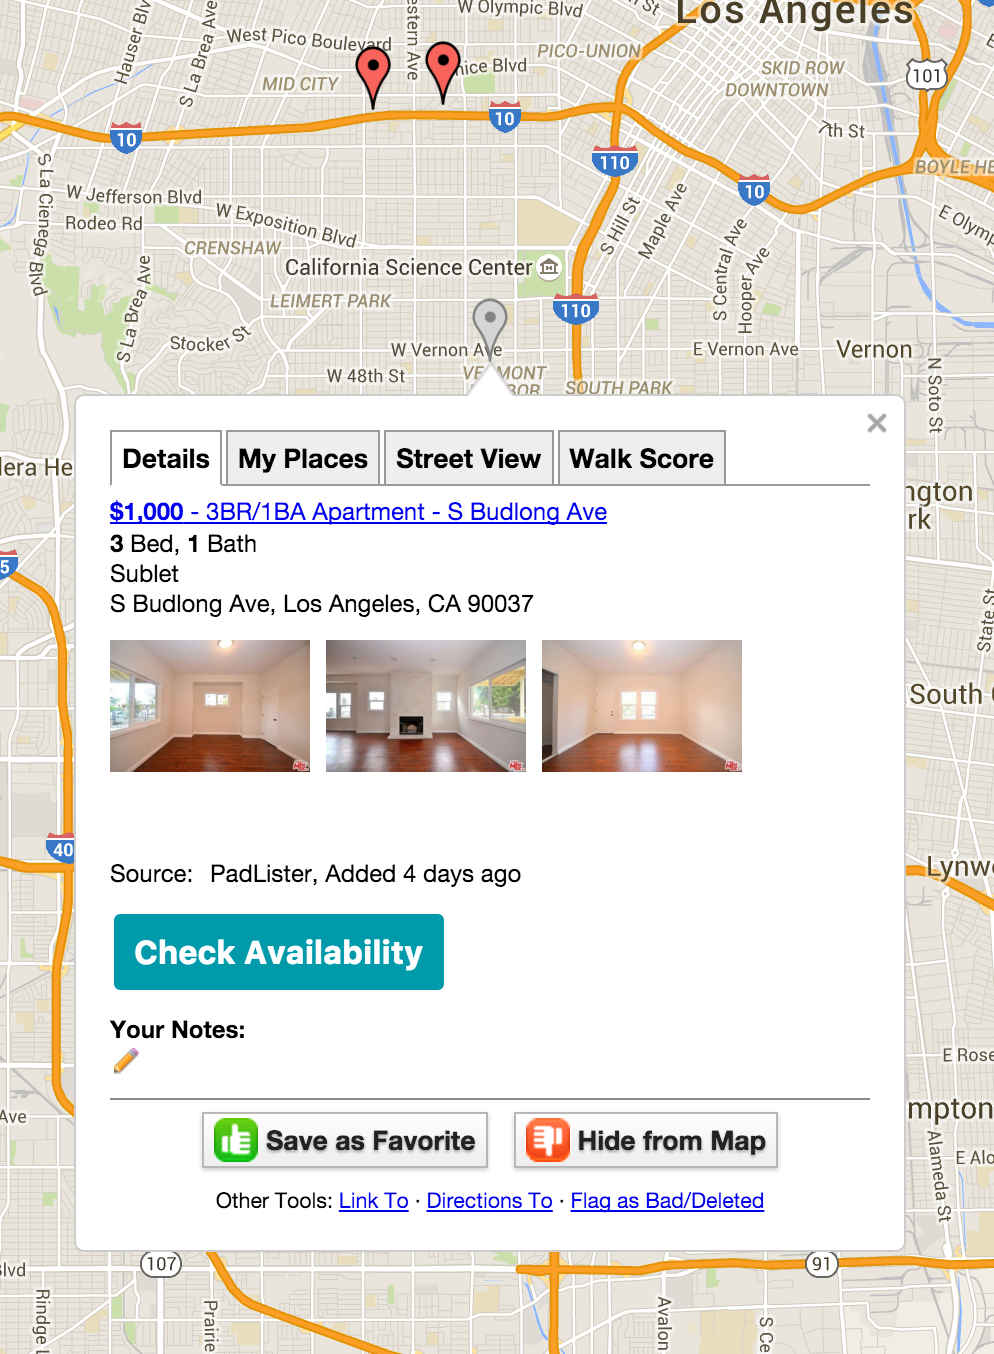
\includegraphics[width=7cm]{markerBox}
    \caption{A marker displaying the information it contains in a box}
    \label{fig:markerDisplay}                
\end{figure}

Note: the paragraph below also applies to what the Tweets would visually appear like in the "Tweets" section, and as it is written here, will not be reiterated again. The tweet organization should be minimal and similar to what is currently implemented. All the data will be stored in a white box. The user profile will be far left with subtle rounded corners. Padded from the left, and from the right. Padding top would be aligned with the padding of the username, which would be to the right of the image (containing some padding between image). The user's name will be bolded. The user's ID will be on the same line as their name, separated by a space, but in smaller font that is grey. After the user ID, the time the tweet was posted would be displayed, also in grey font and smaller size. Below this line, the actual tweet will be seen. It is important to differentiate the elements stylistically so that a user can quickly see and differentiate all of the items (i.e. differentiating the username from the user ID, time posted, and the tweet content). Please see figure~\ref{fig:tweetExample} for what the tweet should look like.

\begin{figure}[H]
    \centering
    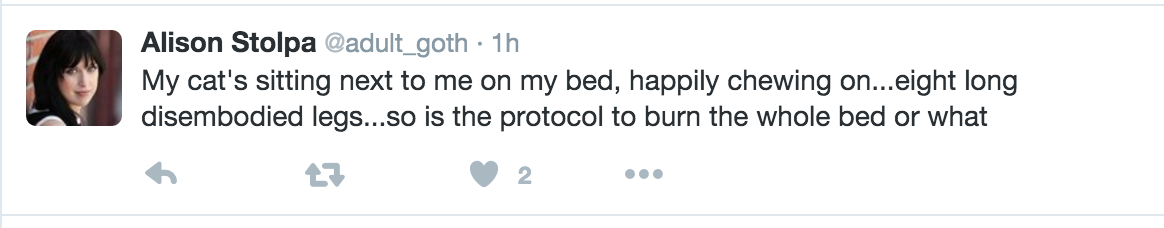
\includegraphics[width=20cm]{tweetExample}
    \caption{An example of a tweet's appearance}
    \label{fig:tweetExample}                
\end{figure}

Notice the ability to interact with the tweet. A user should be able to tweet, retweet, save, delete and direct message the user. Basic principles of presentation are being incorporated, with bold text attracting the user's eye, grey and harder to see text not being as important. A minimal approach for a sleek look is the goal, with just a thin grey line to separate all the tweets. During testing, attempts to make the boxes more colorful were made, but they were far too distracting.

\subsubsection{Marker States}
Similar to general button guidelines, markers should be in obvious states based on what the user has done. At first, all markers will be of the same color, let's for now assume that color will be red. Once a user taps on a tweet, the marker turns grey, to indicate it was already viewed. If a user decides to delete a tweet, it will remove it form the map, and from the Tweet list. If a user decided to save the tweet, the marker will now glow gold. The ability to delete the tweet will be locked, and it will only be deletable after the user removes the star.

\subsubsection{Force Touch Implementation}
Force touch should also be implemented, so that if a user hard-presses on a marker, it instantaneously shows them all the information, and the larger box that can be interacted with. A soft tap will display the smaller box.

\subsubsection{Searching Map Location}
If a user doesn't know the address of a location, he should still be able to search it. There would be an unobstructive button in the top right corner of the map that says "search map location". If pressed, this would automatically jump to the search page. A thin banner at the top would display "map location saved for search", and it would disappear after 5 seconds. Now, when the user searches, the center location of the map that he had shown on the device would the location searched, and the radius would be the furthest distance from the center to an edge of the screen. This could be easily cleared in the advanced settings if the user wanted to return to searching their current location.

\subsection{Tweets}
Tweets are at the core of this app. When on the tweets page, it will simply display each tweet and all their information in white boxes, and approximately 4 to 5 tweets should be seen on the screen. the user can then scroll through the list to see what they found.

Tweet layouts should be simple, minimal, and easy to distinguish. All data pulled from the API should be properly structured. Please see Markers Storing Data section for a description and an image of what the tweets should appear like. The same functionality of smaller and larger boxes will be incorporated to reduce clutter on the page.


\subsubsection{Deleting/Saving Tweet Results}
The ability to flick individual tweets that are of no interest should also be implemented. That way, if a user gets 100 tweets back from their search, if one or some of them are of interest to them, they can swipe it left, which would not only remove the tweet from the list, but also remove a marker on the map associated to it. On the other end of the spectrum, they should be able to save tweets so that they can interact with them later, by swiping right. This would be saved and found under their "profile" tab. That way, they can at a later time share the tweet with friends, retweet it, direct message the user, or simply save it for whatever reason they want. Visually, this would look identical to the process of deleting or archiving mail on most mail apps, and would be accompanied by two different noises for each action. See Figure~\ref{fig:swipeDelete}.

\begin{figure}[H]
    \centering
    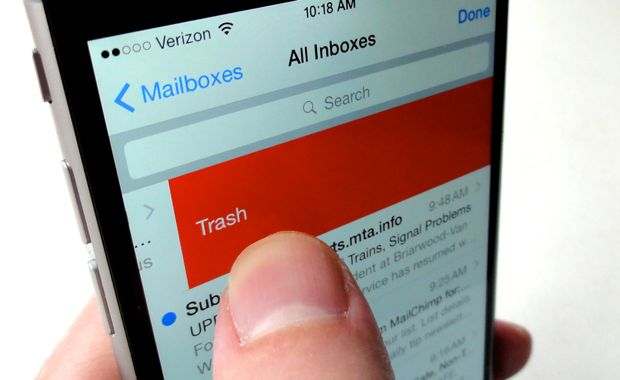
\includegraphics[width=7cm]{swipeDelete}
    \caption{Swiping to delete}
    \label{fig:swipeDelete}
\end{figure}

In case it is not obvious, as the user swipes, the entire box that contains the tweet would slide in a color (red or blue, depending on which action is occurring), and the more they swipe, the more the color slides in, until they finally reach the edge of the screen, on release, the tweet would be deleted/saved.

\subsubsection{Map Integration}
Navigating between tweets and the map page should be effortless and streamlined. A user should be able to press on a tweet (at the moment, I am thinking that pressing anywhere in the tweet box would bring you to the map, but I also want to test having a button that says "Show on map" within the tweet box. The problem with the "Show on map" is that every tweet will have it, and it will dirty up the screen, but if it is not there, the learnability of tapping on a tweet to get to the map part will be bad, as it is not an apparent action). Just like markers turning grey once a user presses on one, the same would happen for the tweets in the list. The box would change colors to clearly show the user has already looked up that tweet. And similarly to the gold hue to a marker if the user saved the tweet, the box containing the tweet information would turn gold to indicate that it is a saved tweet, and swiping to delete it will not be possible.

\subsubsection{Clumping Tweets}
Since sometimes Twitter's results will have users who tweet more than once for the requested search word, clumping their tweets together would make the results easier to traverse. A small plus sign would be placed to the top left of their tweet box, when pressed, their username, photo, and name would remain in a box, but the height would be smaller, and then multiple smaller boxes, indented by half an inch from the left, to visualize they belong to that one user, would only display the tweet and time of the tweet. This should be on by default, but in advanced settings, users could disable this.

\subsubsection{Interacting with Tweets}
As mentioned before, there are several ways to interact with tweets. Aside for swiping to delete/save tweets (or tapping on links like the user ID or links within the tweet), the app user should be able to retweet, direct message, or just simply tweet from within the app. If a user pushes on either the retweet, direct message, or tweet buttons that appear in the bottom of the tweet box, a  flat box would appear, making everything else around it fuzzy, exactly like ForceTouch on the iPhone. Please see figure~\ref{fig:tweetInteraction}

\begin{figure}[H]
    \centering
    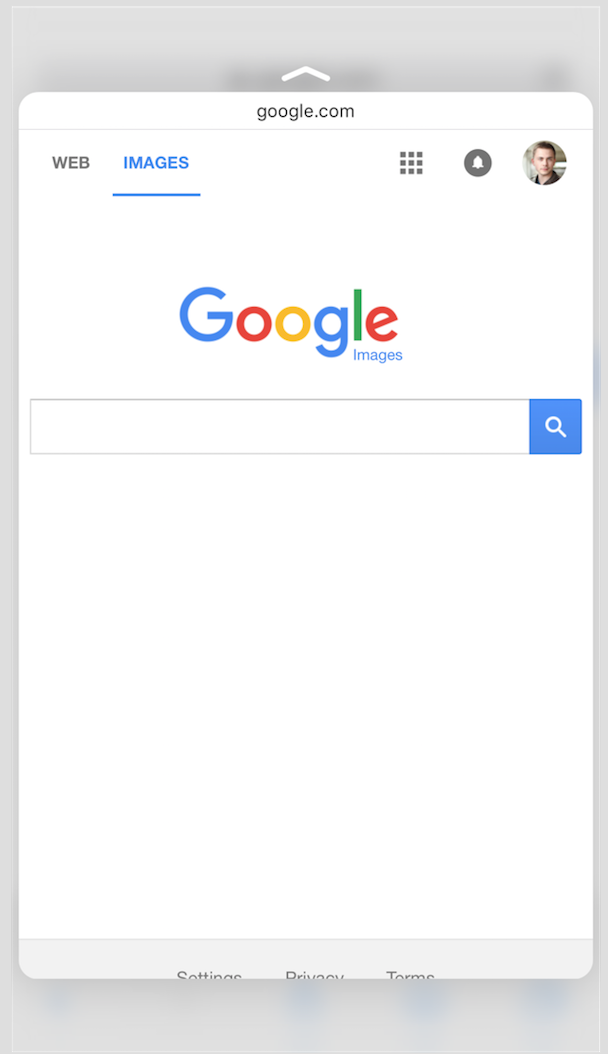
\includegraphics[width=5cm]{tweetInteractionImage}
    \caption{Interactive pop-up box}
    \label{fig:tweetInteraction}
\end{figure}

The data inside the box(text field, user picture, hashtags, etc) would take up about two thirds of the box, leaving one third of the space for the keyboard. To close the box, the user could either tap outside of the box, or flick it up or down. Flicking up or down would have the box fly out of view either towards the top, or bottom of the screen, depending on the flick direction, and the fuzzy effect would dissipate. This is so the user feels like he is manipulating something in real life, if they throw a ball in a direction, the ball would of course move in the direction it was thrown.

The content of the box would look essentially identical to the tweet app's retweet button. Please see figure~\ref{fig:TweetInteractionBoxAppearance}


\begin{figure}[H]
    \centering
    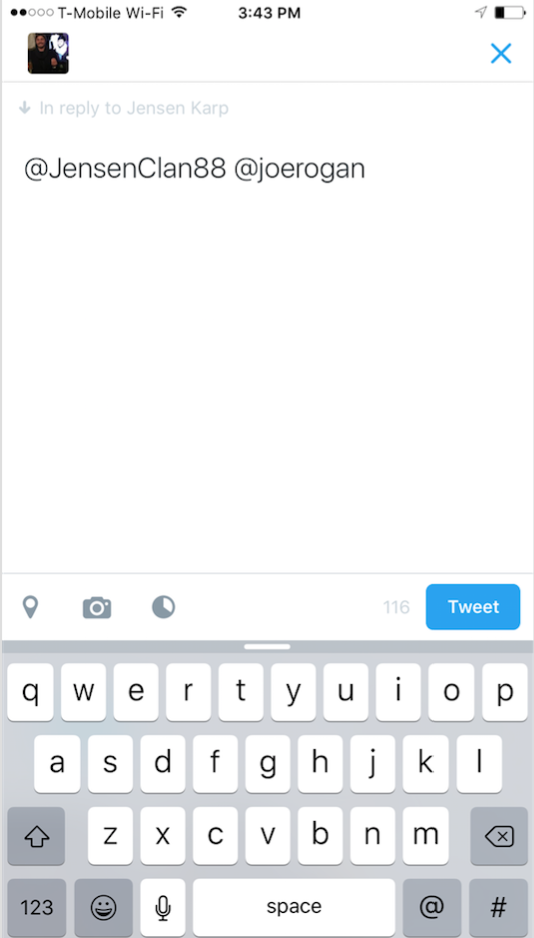
\includegraphics[width=7cm]{retweetBox}
    \caption{Appearance of the tweet/retweet/direct message box}
    \label{fig:TweetInteractionBoxAppearance}
\end{figure}

Tweeting and retweeting would look the same, but sending a direct message would just change the ``Tweet" button text to ``Send".

If a user has not logged in to their Twitter account, and are using the guest account, they would be prompted to login anytime they tried saving, deleting, or interacting with tweets.

\section{Profile}
The profile section will have a list of all the tweets saved by the user. There will also be a button in the top right corner. This button would resemble a map, with the text ``Map them" overlaying the image. When pressed, it would jump to the maps page. If the user had previously done a search and still has pins, it would ask them if they are sure they want to start a new search. If they accept (or did not have a previous search), it would drop all their saved tweets on the map, represented by gold markers. Only in the profiles section could users unsave tweets, to guarantee no accidental deletions. This allows the user to easily see their saved tweets that matter to them, both in map and list form. The profiles section will also save their custom update results. Please see next section for more details on custom updates.

\section{Extra Functionality}
If users want to be updated about tweets when outside the app, they can enable custom updates, under settings, accessible from the sandwich navbar menu. They can set time intervals, and so for example, every hour, they would get a banner that appears on their phone that tells them how many new tweets in their designated area and radius have appeared while they were not using the app. For example, a banner would appear saying ``There have been 25 new tweets regarding Kobe Bryant within a mile of the Staples Center". If the banner is clicked on, it will take them to the Tweets page, which would have generated all the new tweets. The map page would have updated dropped markers. The results are saved under their Profile page, so that if they do not see the update or don't click on the banner, they can see it at a later time.

\section{Usage Scenarios}
The main appeal of the app will be much more clear once users test it extensively, and feedback is provided. For now, here are some examples of how the app can be used:

\begin{itemize}
\item A promoter getting updates on who's talking about his venue. They will get feedback seeing if people are enjoying it, and which musician/DJ/artist is the most tweeted.
\item Artists looking where to provide their next show. This could be musicians, stand ups, singers, etc. If people are tweeting about them in a particular area, they can plan their next show around that. A great way to figure out where their fans are. This is especially useful if they are looking in other states or countries, as they don't have much reach to gather information from such a far distance.
\item Finding a job. The web application alpha release has already had a user acquire a job using Tweet District. They searched ``hiring" within a mile radius, and found a position matching their needs.
\item Finding sales. If a user is shopping around, they can search specific words that will show them if local stores are having promotions.
\item Discovering your neighborhood. If you are new or just want to know what is happening, you can look up events based on custom or predefined search words to figure out if there is a parade, community event, etc.
\item Finding parties or bars. College students can look up parties near campus, others can look up where people are tweeting about bars or are having the most fun, to choose an exciting venue. In fact, during alpha testing, a few users found a red carpet after-party using Tweet District, and ended up going. They claimed it was very exciting and fun.
\end{itemize}

As a one liner, the purpose is to allow people to discover their surrounding areas by scraping data from social media, for a more intertwined community.

\section{Usability Metric Forecast}
Learnability, efficiency, errors, memorability, and satisfaction are usability metrics. 

In terms of importance, satisfaction, and efficiency are of utmost priority. The app should navigate smoothly, and search results should occur almost instantaneously. Users should of course enjoy the process, as well as the results they find. If they do not experience satisfaction, they would cease to use the app. There should be no hang time navigating between pages, and all animations should be smooth. 

A little lower on the spectrum would be learnability and memorability. For the basic functions, learnability should be quick with almost no learning curve. It should be simple enough to search a word, see results, and see the markers on the map that represent these results. It is okay and expected for more advanced features to have a steeper learning curve, and wouldn't  be much of a detriment if users have to consult the FAQ to get more information on some of the features, such as advanced searching, deleting tweets, and so forth. Memorability after some time away from the app should be the same, as for the simple functions, remembering shouldn't be a problem, but with more advanced features, a quick read in the FAQ will not cause any damage to the user experience.

User errors are placed at the bottom of the importance ladder. There should however, be very little of them, as this would cause frustration, and would taint their satisfaction. It is important to note that user errors are not detrimental in terms of serious repercussions. It is not a program that is guiding a NASA spaceship, or a tax company's auditing software; those kinds of errors would be of utmost importance and would take high priority. Although this app can be used for commercial purposes, such as gathering data about clients or who is tweeting about your business, some errors are okay. Again, the main concern would be user satisfaction.


\section{Overall design}
Firstly, I would like to directly steal Apple's new standard font, and, as they say, ``The system font is a specially optimized version of Helvetica Neue, which displays textual content with beauty, clarity, and sharpness." In terms of colors, I want to keep it light and fun. I've been trying to find some color palettes, and since it's Twitter, I am thinking a light blue should be involved.  Below are two color palette ideas to represent the app's intention. No dark colors, all fun, light, vibrant colors. I also definitely wanted to have another color that stands out. For now it's a bright orange for the logo that counter-acts the mainly white and blue remainder of the web app. See Figure~\ref{fig:palette} below for color palette samples.

\begin{figure}[H]
    \centering
    \subfloat[Palette 1]{{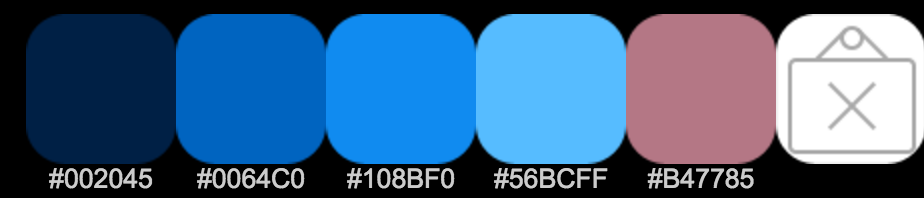
\includegraphics[width=9cm]{palette1} }}
    \qquad
    \subfloat[Palette 2]{{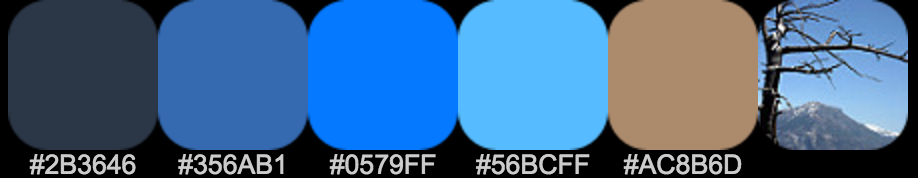
\includegraphics[width=9cm]{palette2} }}
    \caption{Potential Color Palettes}
    \label{fig:palette}          

\end{figure}

The overall design should have a flat, clean layout. Similar to Apple, I want very subtle rounded corners on boxes, buttons and panels. In terms of animations, I do not want them to be gratuitous. They are meant to mimic realistic motion, such as sliding left and right, and flicking open boxes (larger boxes for tweets as mentioned earlier, when retweeting/direct messaging/tweeting box pops up, etc). The goal in dividing the functionality into three separate, but quick and easy to switch categories (Tweets, Map, Search) is to enhance user flow.

Below is the current Tweet District color combinations, and I think they work. Perhaps changing the logo/brand to a slightly different, but similar color. Large bolder text to represent sections, smaller, grayer text for a slogan. Bolded text to attract attention to key parts, and a subtle navbar with a bit of transparency to it. See Figure~\ref{fig:currentPalette} (zooming in on the below image is recommended).


\begin{figure}[H]
    \centering
    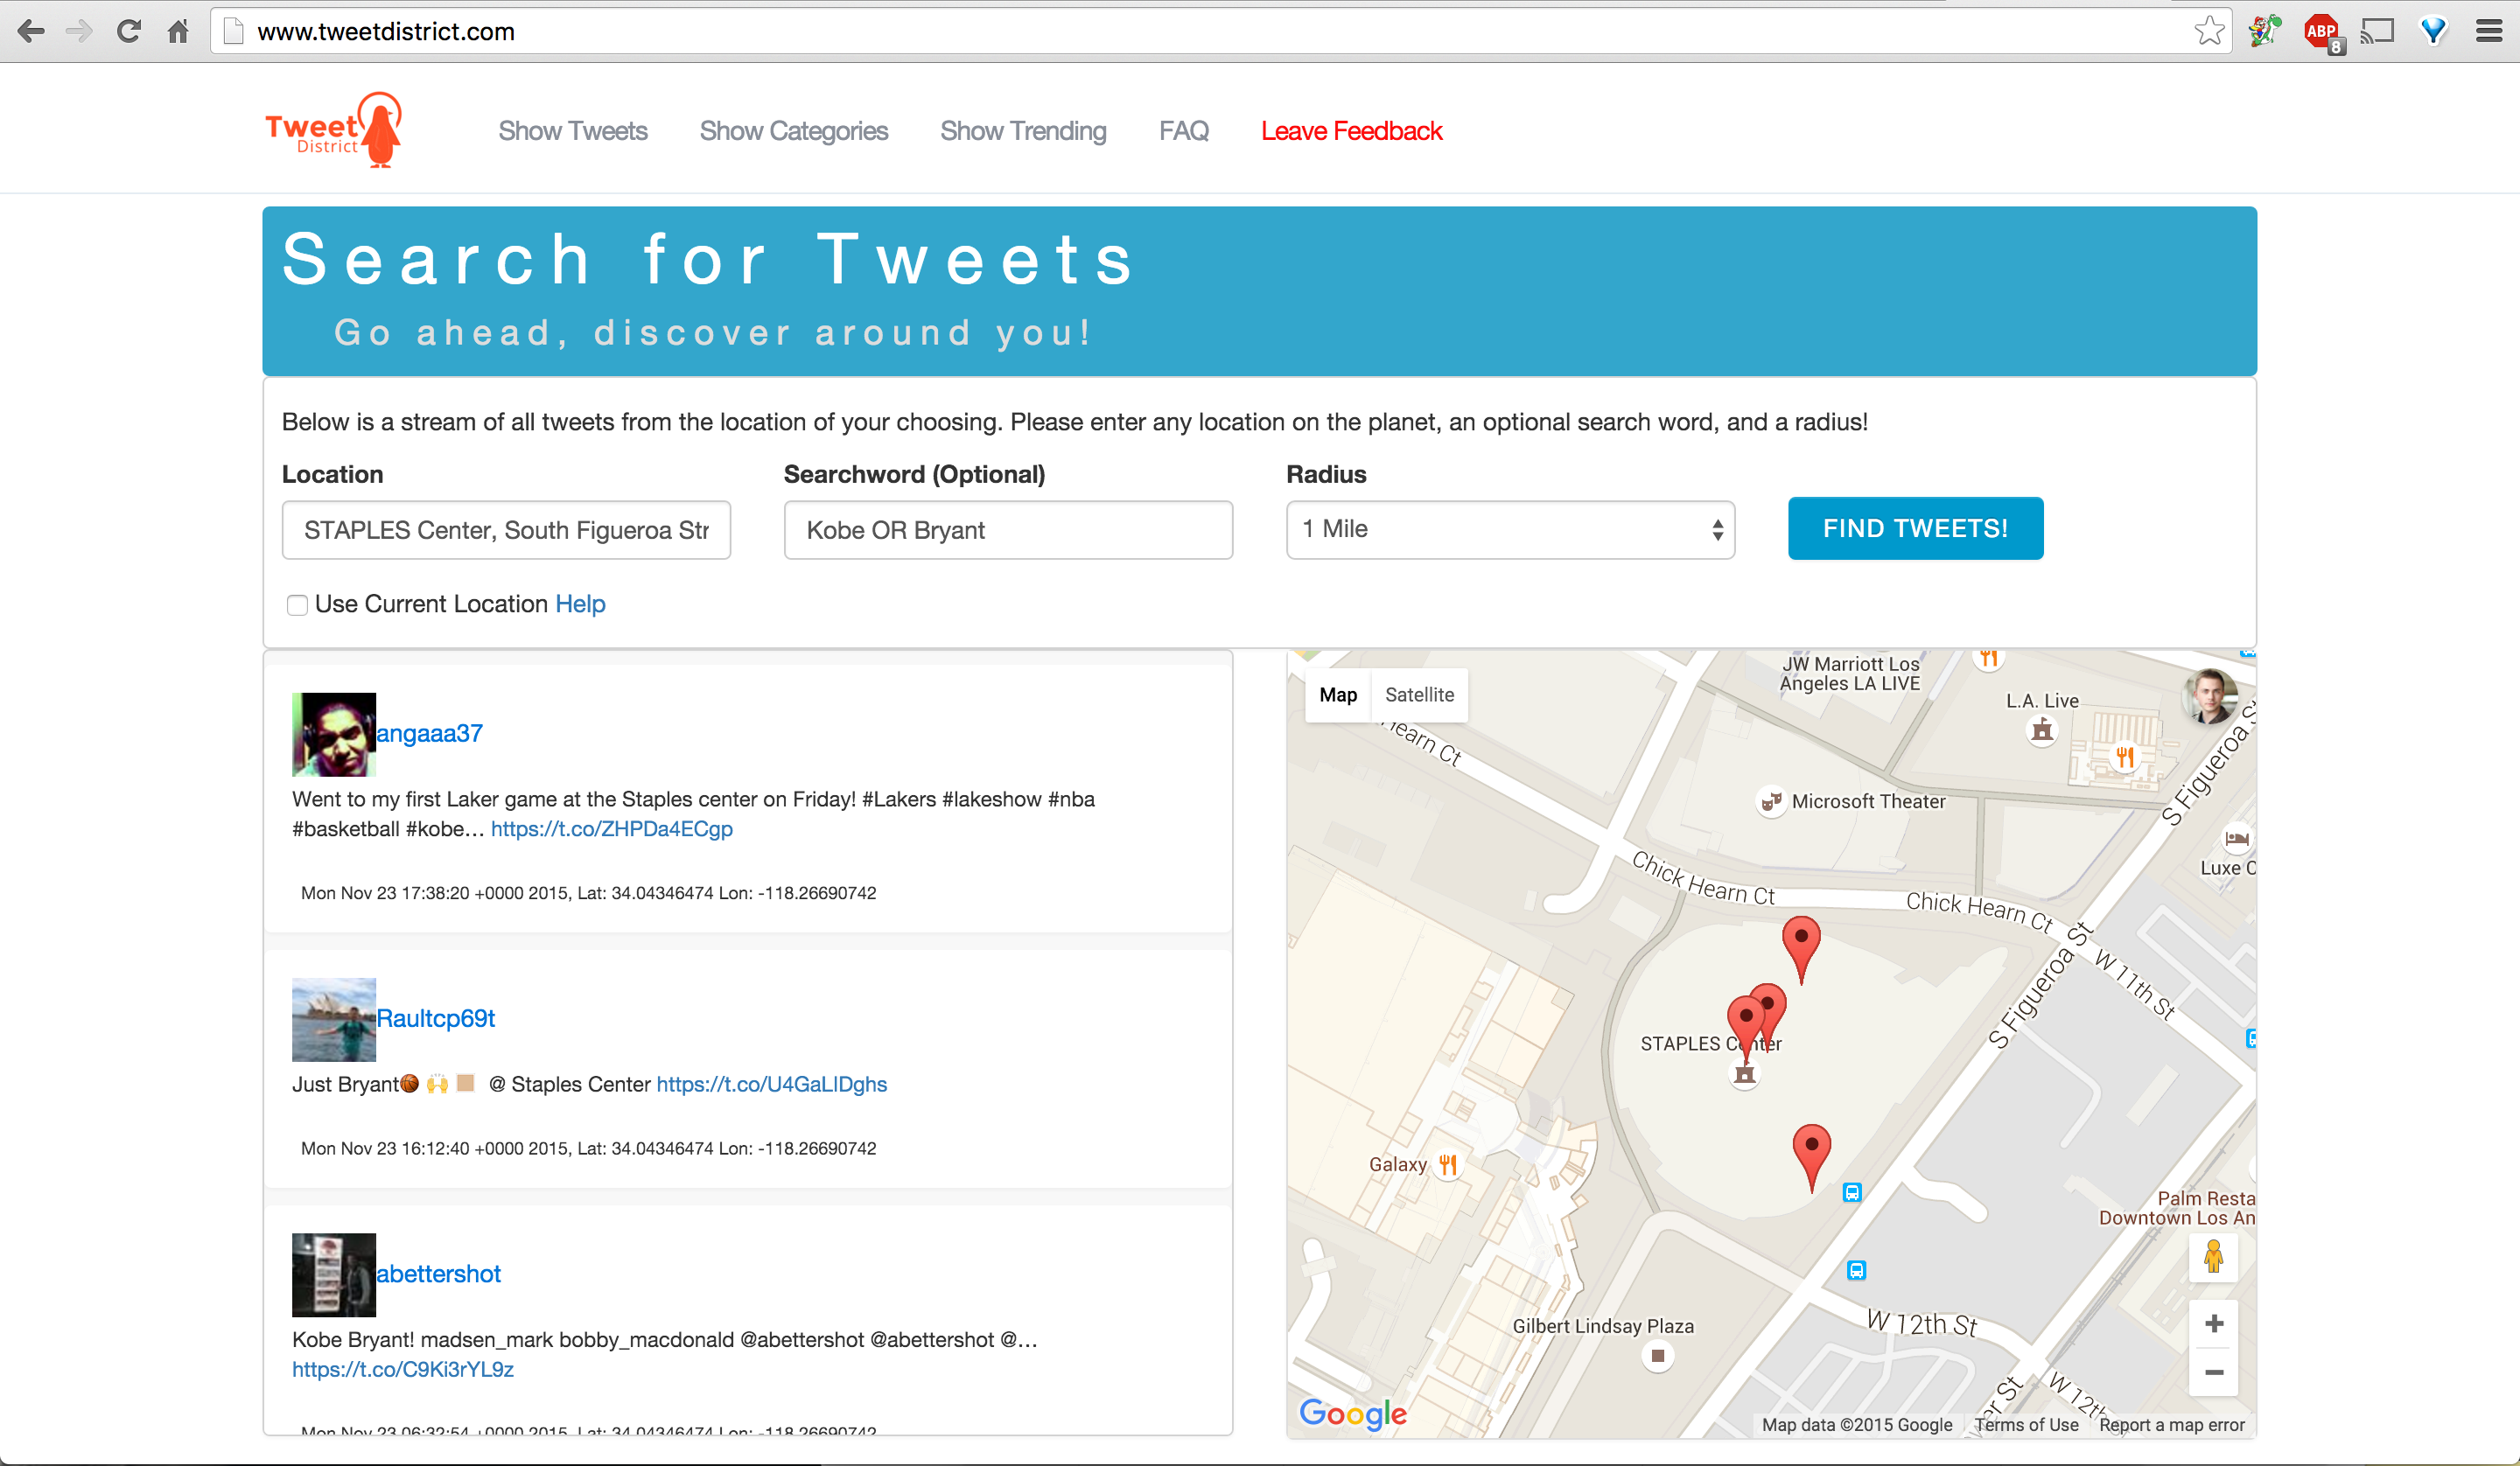
\includegraphics[width=15cm]{currentPaletteSample}
    \caption{Current colors of Tweet District Web Application}
    \label{fig:currentPalette}
\end{figure}

\end{document}
